\setcounter{chapter}{2}
\chapter{The Definition of Groups}
\label{ch:the-definition-of-groups}
%% FIXME: \cite{Pinter2016}*{Chapter 3}

\begin{enumerate}[label={\Alph*.},font={\bfseries}]
\item {\bf Examples of Abelian Groups}
  \begin{enumerate}[label={\arabic*},font={\bfseries}]
  \item $\Group{\mathbb{R}, x*y=x+y+k}$
    \begin{enumerate}[label={(\roman*)}]
    \item $*$ is commutative:
      $x*y=x+y+k = y+x+k=y*x$
    \item $*$ is associative.
      \begin{alignat*}{3}
        & x(yz) &&= x(y+z+k) &&= x+y+z+2k \\
        & (xy)z &&= (x+y+k)z &&= (xy)z \\
        & x(yz) &&= (xy)z
      \end{alignat*}
    \item $\mathbb{R}$ has an identity element with respect to $*$.
      \begin{align*}
        xe &= x \\
        x+e+k &= x \\
        e &= -k \\
        (-k)x &= x \\
        -k+x+k &= x
      \end{align*}
    \item $\forall x\in\mathbb{R}(\exists x^\prime\in\mathbb{R}(x*x^\prime=-k))$
      \begin{alignat*}{3}
        xx^\prime &= -k \\
        x+x^\prime+k &= -k \\
        x^\prime &= -x-2k \\
        x^{\prime}x &= xx^\prime & \text{due to commutativity}
      \end{alignat*}
    \end{enumerate}
  \item $\Group{\mathbb{R}^*, x*y=\frac{xy}{2}}$
    \begin{enumerate}[label={(\roman*)}]
    \item $*$ is commutative:
      $x*y=\frac{xy}{2} = \frac{yx}{2}=y*x$
    \item $*$ is associative.
      \begin{alignat*}{3}
        x*(y*z) &= x*(\frac{yz}{2}) &= \frac{xyz}{4} \\
        (x*y)*z &= (\frac{xy}{2})*z &= \frac{xyz}{4}
      \end{alignat*}
    \item $\mathbb{R}^*$ has an identity element with respect to $*$.
      \begin{align*}
        x*e &= \frac{xe}{2} = \frac{ex}{2}=e*x = x \\
        e &= 2
      \end{align*}
    \item $\forall x\in\mathbb{R}(\exists x^\prime\in\mathbb{R}(x*x^\prime=2))$
      \begin{align*}
        x*x^\prime &= \frac{xx^\prime}{2} = \frac{x^{\prime}x}{2} = x^{\prime}*x = e = 2 \\
        x^\prime = \frac{4}{x}
      \end{align*}
    \end{enumerate}
  \item $\Group{\Set{x\in\mathbb{R} : x \neq -1}, x*y=x+y+xy}$
    \begin{enumerate}[label={(\roman*)}]
    \item $*$ is commutative: $x*y=x+y+xy = y+x+yx=y*x$
    \item $*$ is associative.
      \begin{alignat*}{3}
        x*(y*z) &= x*(y+z+yz) = x+(y+z+yz)+x(y+z+yz) &= x+y+z+xy+xz+yz+xyz \\
        (x*y)*z &= (x+y+xy)*z = (x+y+xy)+z+(x+y+xy)z &= x+y+z+xy+xz+yz+xyz
      \end{alignat*}
    \item $\Set{x\in\mathbb{R} : x \neq -1}$ has an identity element with respect to $*$.
      \begin{align*}
        x*e &= x+e+xe = e+x+ex = e*x = x \\
        e(x+1) &= 0 \\
        e &= 0
      \end{align*}
    \item Every element of $\Set{x\in\mathbb{R} : x \neq -1}$ has an inverse with respect to $*$.
      \begin{align*}
        x*x^\prime &= x+x^\prime+xx^\prime=x^\prime+x+x^{\prime}x = e = 0 \\
        x^{\prime}(x+1) &= -x \\
        x^\prime &= -\frac{x}{x+1}
      \end{align*}
    \end{enumerate}
  \item $\Group{\Set{x\in\mathbb{R} :-1 < x < 1}, x*y=\frac{x+y}{xy+1}}$
    \begin{enumerate}[label={(\roman*)}]
    \item $*$ is commutative: $x*y=\frac{x+y}{xy+1}=\frac{y+x}{yx+1}=y*x$
    \item $*$ is associative.
      \begin{alignat*}{4}
        x*(y*z) &= x*(\frac{y+z}{yz+1})
        &= \frac{x+(\frac{y+z}{yz+1})}{x(\frac{y+z}{yz+1})+1}
        &= \frac{xyz+x+y+z}{xy+xz+yz+1} \\
        (x*y)*z &= \frac{x+y}{xy+1}*z
        &= \frac{(\frac{x+y}{xy+1})+z}{(\frac{x+y}{xy+1})z+1}
        &= \frac{x+y+z+xyz}{xy+yz+xz+1}
      \end{alignat*}
    \item $\Set{x\in\mathbb{R} : -1 < x < 1}$ has an identity element w.r.t. $*$.
      \begin{align*}
        x*e &= \frac{x+e}{xe+1} = x \\
        x+e &= x(xe+1) \\
        e &= ex^2 \\
        e(1-x^2) &= 0 \\
        e &= 0 \\
        x*0 &= \frac{x+0}{(x\times0)+1} = x = \frac{0+x}{0x+1} = 0*x
      \end{align*}
    \item Every element of $\Set{x\in\mathbb{R} : -1 < x < 1}$ has an inverse with respect to $*$.
      \begin{align*}
        x * x^\prime &= \frac{x+x^\prime}{xx^\prime+1} = 0; \quad
        x+x^\prime = 0; \quad
        x^\prime = -x \\
        x*(-x) &= \frac{x-x}{x(-x)+1} = 0 = \frac{-x+x}{-x^2+1} = (-x)*x
      \end{align*}
    \end{enumerate}
  \end{enumerate}
\item {\bf Groups on the Set $\mathbb{R} \times \mathbb{R}$}
  \begin{enumerate}[label={\arabic*},font={\bfseries}]
  \item $(a,b) * (c,d) = (ad + bc, bd)$, on the set $\Set{(x,y)\in\mathbb{R}\times\mathbb{R} : y \ne 0}$
    \begin{enumerate}[label={(\roman*)}]
    \item $*$ is commutative.
      \begin{align*}
        (c,d) * (a,b) &= (cb+da,db) \\
        &= (ad+bc,bd) \\
        &= (a,b) * (c,d)
      \end{align*}
    \item $*$ is associative.
      \begin{align*}
        (a,b) * \left[(c,d) * (e,f)\right] &= (a,b) * (cf+de,df) \\
        &= (adf+bcf+bde,bdf) \\
        &= (ad+bc, bd) * (e,f) \\
        &= \left[(a,b) * (c,d)\right] * (e,f)
      \end{align*}
    \item $(e_1,e_2) = (0,1)$
      \begin{align*}
        (a,b) * (e_1,e_2) &= (ae_2 + be_1, be_2) \\
        &= (a,b) \\
        \\
        be_2 &= b \\
        e_2 &= 1 \\
        \\
        ae_2 + be_1 &= a \\
        a + be_1 &= a \\
        e_1 &= 0
      \end{align*}
    \item $(a^\prime,b^\prime) = \left(\frac{-a}{b^2}, \frac{1}{b}\right)$
      \begin{align*}
        (a,b) * (a^\prime,b^\prime) &= (ab^\prime + ba^\prime, bb^\prime) \\
        &= (0,1)
      \end{align*}
      \begin{align*}
        bb^\prime &= 1 \\
        b^\prime &= \frac{1}{b} \\
        \\
        ab^\prime + ba^\prime &= 0 \\
        \frac{a}{b} + ba^\prime &= 0 \\
        ba^\prime &= \frac{-a}{b} \\
        a^\prime &= \frac{-a}{b^2} \\
        \\
        (a,b) * \left(\frac{-a}{b^2}, \frac{1}{b}\right) &= \left(\frac{a}{b} + \frac{-a}{b}, b\left(\frac{1}{b}\right)\right) \\
        &= (0,1)
      \end{align*}
    \end{enumerate}
  \item $(a, b) * (c, d) = (ac, bc + d)$, on the set $\Set{(x,y)\in\mathbb{R}\times\mathbb{R} : x \ne 0}$
    \begin{enumerate}[label={(\roman*)}]
    \item $*$ is not commutative: $(c,d) * (a,b) = (ca, da + b) \ne (a,b) * (c,d)$
    \item $*$ is associative.
      \begin{align*}
        \left[(a,b) * (c,d)\right] * (e,f) &= (ac, bc+d) * (e,f) \\
        &= (ace, bce+de+f) \\
        &= (a,b) * (ce, de+f) \\
        &= (a,b) * \left[(c,d) * (e,f)\right]
      \end{align*}
    \item $(e_1,e_2) = (1,0)$
      \begin{align*}
        (a,b) * (e_1,e_2) &= (ae_1, be_1+e_2) \\
        &= (a, b) \\
        \\
        ae_1 &= a \\
        e_1 &= 1 \\
        \\
        be_1+e_2 &= b \\
        b+e_2 &= b \\
        e_2 &= 0
      \end{align*}
    \item $(a^\prime,b^\prime) = (\frac{1}{a},\frac{-b}{a})$
      \begin{align*}
        (a,b) * (a^\prime,b^\prime) &= (aa^\prime, ba^\prime + b^\prime) \\
        &= (1,0) \\
        \\
        aa^\prime &= 1 \\
        a^\prime &= \frac{1}{a} \\
        \\
        ba^\prime + b^\prime &= 0 \\
        \frac{b}{a} + b^\prime &= 0 \\
        b^\prime &= \frac{-b}{a}
        \\
        (a,b) * (\frac{1}{a}, \frac{-b}{a}) &= (\frac{a}{a}, \frac{b}{a} - \frac{b}{a}) \\
        &= (1,0)
      \end{align*}
    \end{enumerate}
  \item $(a, b) * (c, d) = (ac, bc + d)$, on the set $\Set{(x,y)\in\mathbb{R}\times\mathbb{R}}$
    \begin{enumerate}[label={(\roman*)}]
    \item $*$ is not commutative, as per 2(i).
    \item $*$ is associative, as per 2(ii).
    \item $(e_1,e_2) = (1,0)$, as per 2(iii).
    \item $a^\prime$ is not defined $\forall a\in\mathbb{R}$, notably when $a=0$.
    \end{enumerate}
  \item $(a, b) * (c, d) = (ac-bd,ad+bc)$, on the set $\Set{(x,y)\in(\mathbb{R}\times\mathbb{R})\setminus\Set{(0,0)}}$
    \begin{enumerate}[label={(\roman*)}]
    \item $*$ is commutative.
      \begin{align*}
        (c,d) * (a,b) &= (ca-db,cb+da) \\
        &= (ac-db,ad+bc) \\
        &= (a,b) * (c,d)
      \end{align*}
    \item $*$ is associative.
      \begin{align*}
        (a,b) * \left[(c,d) * (e,f)\right] &= (ac-bd,ad+bc) * (ce-df,cf+de) \\
        &= \left(a(ce-df) - b(cf+de), a(cf+de)+b(ce-df)\right) \\
        &= (ace-adf-bcf-bde, acf+ade+bce-bdf) \\
        &= \left(e(ac-bd)-f(ad+bc), f(ac-bd)+e(ad+bc)\right) \\
        &= (ac-bd,ad+bc) * (e,f) \\
        &= \left[(a,b) * (c,d)\right] * (e,f)
      \end{align*}
    \item $(e_1,e_2) = (1 - \frac{ae_2}{b},\frac{ae_1-a}{b})$
      \begin{align*}
        (a,b) * (e_1,e_2) &= (ae_1-be_2,ae_2+be_1) \\
        &= (a,b) \\
        \\
        ae_2+be_1 &= b \\
        be_1 &= b - ae_2 \\
        e_1 &= 1 - \frac{ae_2}{b} \\
        \\
        ae_1-be_2 &= a \\
        -be_2 &= a-ae_1 \\
        be_2 &= ae_1-a \\
        e_2 &= \frac{ae_1-a}{b}
      \end{align*}
    \end{enumerate}
    \item \todo[inline]{Consider whether $(a, b) * (c, d) = (ac, bc + d)$, on the set $\Set{(x,y)\in\mathbb{R}\times\mathbb{R}}$ is a group.}
  \end{enumerate}
  %% \newpage
\item {\bf Groups of Subsets of a Subset}
  \begin{enumerate}[label={\arabic*},font={\bfseries}]
  \item The identity element with respect to the operation $+$ is $\emptyset$.
    \begin{align*}
      A+I &= (A-I) \cup (I-A) = A \\
      &= (A-\emptyset) \cup (I-\emptyset) \\
      \\
      I &= \emptyset
    \end{align*}
  \item $\Group{\powerset{D}, +}$ is a group, since
    $\forall A \in \powerset{D}, A\inverse = A$.
    \begin{align*}
      A+A\inverse &= \emptyset \\
      (A-A\inverse) \cup (A\inverse-A) &= \emptyset \\
      A-A\inverse &= A\inverse-A = \emptyset \\
      A\inverse &= A
    \end{align*}
  \item Let $D = \Set{a,b,c}$.
    \[
    \powerset{D} = \Set{
      \emptyset,
      \Set{a}, \Set{b}, \Set{c},
      \Set{a,b}, \Set{a,c}, \Set{b,c},
      \Set{a,b,c}
    }
    \]
    \begin{center}
      \captionof{table}{$\Group{\powerset{D}, +}$}
      \begin{tabular}{ c | c c c c c c c c}
        $+$ & $\emptyset$ & $\Set{a}$ & $\Set{b}$ & $\Set{c}$ & $\Set{a,b}$ & $\Set{a,c}$ & $\Set{b,c}$ & $\Set{a,b,c}$ \\
        \hline
        $\emptyset$ & $\emptyset$ & $\Set{a}$ & $\Set{b}$ & $\Set{c}$ & $\Set{a,b}$ & $\Set{a,c}$ & $\Set{b,c}$ & $\Set{a,b,c}$ \\
        $\Set{a}$ & $\Set{a}$ & $\emptyset$ & $\Set{a,b}$ & $\Set{a,c}$ & $\Set{b}$ & $\Set{c}$ & $\Set{a,b,c}$ & $\Set{b,c}$ \\
        $\Set{b}$ & $\Set{b}$ & $\Set{a,b}$ & $\emptyset$ & $\Set{b,c}$ & $\Set{a}$ & $\Set{a,b,c}$ & $\Set{c}$ & $\Set{a,c}$ \\
        $\Set{c}$ & $\Set{c}$ & $\Set{a,c}$ & $\Set{b,c}$ & $\emptyset$ & $\Set{a,b,c}$ & $\Set{a}$ & $\Set{b}$ & $\Set{a,b}$ \\
        $\Set{a,b}$ & $\Set{a,b}$ & $\Set{b}$ & $\Set{a}$ & $\Set{a,b,c}$ & $\emptyset$ & $\Set{b,c}$ & $\Set{a,c}$ & $\Set{c}$ \\
        $\Set{a,c}$ & $\Set{a,c}$ & $\Set{c}$ & $\Set{a,b,c}$ & $\Set{a}$ & $\Set{b,c}$ & $\emptyset$ & $\Set{a,b}$ & $\Set{b}$ \\
        $\Set{b,c}$ & $\Set{b,c}$ & $\Set{a,b,c}$ & $\Set{c}$ & $\Set{b}$ & $\Set{a,c}$ & $\Set{a,b}$ & $\emptyset$ & $\Set{a}$ \\
        $\Set{a,b,c}$ & $\Set{a,b,c}$ & $\Set{b,c}$ & $\Set{a,c}$ & $\Set{a,b}$ & $\Set{c}$ & $\Set{b}$ & $\Set{a}$ & $\emptyset$
      \end{tabular}
    \end{center}
  \end{enumerate}
\item {\bf A Checkerboard Game}
  \begin{center}
    \captionof{table}{$\Group{G, *}$}
    \begin{tabular}{ c | c c c c }
      $*$ & $I$ & $V$ & $H$ & $D$ \\
      \hline
      $I$ & $I$ & $V$ & $H$ & $D$ \\
      $V$ & $V$ & $I$ & $D$ & $H$ \\
      $H$ & $H$ & $D$ & $I$ & $V$ \\
      $D$ & $D$ & $H$ & $V$ & $I$
    \end{tabular}
  \end{center}
  As shown in the \gls{Cayley table} above, the identity element is $I$ and
  every element is its own inverse. Having shown that and granting
  associativity, $\Group{G, *}$ is a group.
\item {\bf A Coin Game}
  \begin{center}
    \captionof{table}{$\Group{G, *}$}
    \begin{tabular}{ c | c c c c c c c c }
      $*$ & $I$ & $M_1$ & $M_2$ & $M_3$ & $M_4$ & $M_5$ & $M_6$ & $M_7$ \\
      \hline
      $I$ & $I$ & $M_1$ & $M_2$ & $M_3$ & $M_4$ & $M_5$ & $M_6$ & $M_7$ \\
      $M_1$ & $M_1$ & $I$ & $M_3$ & $M_2$ & $M_5$ & $M_4$ & $M_7$ & $M_6$ \\
      $M_2$ & $M_2$ & $M_3$ & $I$ & $M_1$ & $M_6$ & $M_7$ & $M_4$ & $M_5$ \\
      $M_3$ & $M_3$ & $M_2$ & $M_1$ & $I$ & $M_7$ & $M_6$ & $M_5$ & $M_4$ \\
      $M_4$ & $M_4$ & $M_6$ & $M_5$ & $M_7$ & $I$ & $M_2$ & $M_1$ & $M_3$ \\
      $M_5$ & $M_5$ & $M_7$ & $M_4$ & $M_6$ & $M_1$ & $M_3$ & $I$ & $M_2$ \\
      $M_6$ & $M_6$ & $M_4$ & $M_7$ & $M_5$ & $M_2$ & $I$ & $M_3$ & $M_1$ \\
      $M_7$ & $M_7$ & $M_5$ & $M_6$ & $M_4$ & $M_3$ & $M_1$ & $M_2$ & $I$
    \end{tabular}
  \end{center}

  As shown in the \gls{Cayley table} above, the identity element is $I$ and
  every element is invertible. Having shown that and granting associativity,
  $\Group{G, *}$ is a group. It is not commutative, because, for example
  $M_6 * M_4 = M_2$, while $M_4 * M_6 = M_1$, so $M_6 * M_4 \ne M_4 * M_6$.
  \newpage
  \captionof{figure}{$\Group{r,s,t\ |\ r^2,s^2,t^2,(rs)^4,(st)^3,(rt)^2}$}
  \begin{figure}[h]
    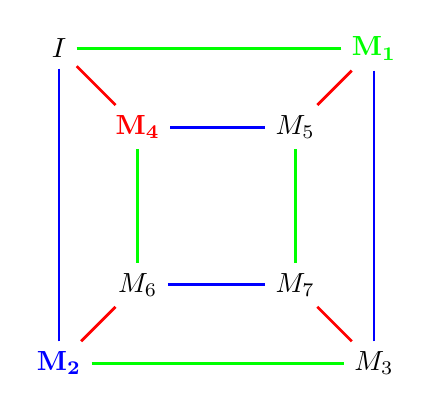
\begin{tikzpicture}[line width=1pt]
      \node (I) at (0,4) { $I$ };
      \node (M3) at (4,0) { $M_3$ };
      \node (M5) at (3,3) { $M_5$ };
      \node (M6) at (1,1) { $M_6$ };
      \node (M7) at (3,1) { $M_7$ };

      \node[green] (M1) at (4,4) { $\mathbf{M_1}$ };
      \node[blue] (M2) at (0,0) { $\mathbf{M_2}$ };
      \node[red] (M4) at (1,3) { $\mathbf{M_4}$ };

      \draw[green] (I)  -- (M1)
                   (M1) -- (I)
                   (M2) -- (M3)
                   (M3) -- (M2)
                   (M4) -- (M6)
                   (M5) -- (M7)
                   (M6) -- (M4)
                   (M7) -- (M5);

      \draw[blue] (I)  -- (M2)
                  (M1) -- (M3)
                  (M2) -- (I)
                  (M3) -- (M1)
                  (M4) -- (M5)
                  (M5) -- (M4)
                  (M6) -- (M7)
                  (M7) -- (M6);

      \draw[red] (I)  -- (M4)
                 (M1) -- (M5)
                 (M2) -- (M6)
                 (M3) -- (M7)
                 (M4) -- (I)
                 (M5) -- (M1)
                 (M6) -- (M2)
                 (M7) -- (M3);
    \end{tikzpicture}
  \end{figure}
\item {\bf Groups in Binary Codes}
  \begin{enumerate}[label={\arabic*},font={\bfseries}]
  \item $\Seq{a_1,a_2,...,a_n} + \Seq{b_1,b_2,...,b_n} = \Seq{b_1,b_2,...,b_n} + \Seq{a_1,a_2,...,a_n}$,
    since the left-hand side is equivalent to $\Seq{a_1+b_1,a_2+b_2,...,a_n+b_n}$,
    which by the commutativity of bit addition is equivalent to $\Seq{b_1+a_1,b_2+a_2,...,b_n+a_n}$,
    which is equivalent to $\Seq{b_1,b_2,...,b_n} + \Seq{a_1,a_2,...,a_n}$.
  \item
    \begin{alignat*}{5}
      &1 + (1 + 1) &&= 1 + 0 &&= 1 &&= 0 + 1 &&= (1 + 1) + 1 \\
      &1 + (1 + 0) &&= 1 + 1 &&= 0 &&= 0 + 0 &&= (1 + 1) + 0 \\
      &1 + (0 + 1) &&= 1 + 1 &&= 0 &&= 1 + 1 &&= (1 + 0) + 1 \\
      &0 + (1 + 1) &&= 0 + 0 &&= 0 &&= 1 + 1 &&= (0 + 1) + 1 \\
      &1 + (0 + 0) &&= 1 + 0 &&= 1 &&= 1 + 0 &&= (1 + 0) + 0 \\
      &0 + (0 + 1) &&= 0 + 1 &&= 1 &&= 0 + 1 &&= (0 + 0) + 1 \\
      &0 + (1 + 0) &&= 0 + 1 &&= 1 &&= 1 + 0 &&= (0 + 1) + 0 \\
      &0 + (0 + 0) &&= 0 + 0 &&= 0 &&= 0 + 0 &&= (0 + 0) + 0
    \end{alignat*}
  \item
    \begin{align*}
      \Seq{a_1,a_2,...,a_n} + \left[\Seq{b_1,b_2,...,b_n} + \Seq{c_1,c_2,...,c_n}\right]
      &= \Seq{a_1,a_2,...,a_n} + \Seq{b_1+c_1,b_2+c_2,...,b_n+c_n} \\
      &= \Seq{a_1+b_1+c_1,a_2+b_2+c_2,...,a_n+b_n+c_n} \\
      &= \Seq{a_1+b_1,a_2+b_2,...,a_n+b_n} + \Seq{c_1,c_2,...,c_n} \\
      &= \left[\Seq{a_1,a_2,...,a_n} + \Seq{b_1,b_2,...,b_n}\right] + \Seq{c_1,c_2,...,c_n}
    \end{align*}
    \item The identity element of $\mathbb{B}^n$, that is, the identity element
      for adding words on length $n$, is $0^n$.
    \item The inverse, with respect to word addition, of any word
      $(a_1,...,a_n)$ is $(a_1,...,a_n)$.
    \item $\mathbf{a} + \mathbf{b} = \mathbf{a} + (-\mathbf{b})$,
      since $\mathbf{b} = -\mathbf{b}$.
      Thus $\mathbf{a} + \mathbf{b} = \mathbf{a} - \mathbf{b}$.
    \item
      \begin{align*}
        \mathbf{a} + \mathbf{b} &= \mathbf{c} \\
        \mathbf{a} + (-\mathbf{b}) &= \mathbf{c} \\
        \mathbf{a} - \mathbf{b} &= \mathbf{c} \\
        \mathbf{a} &= \mathbf{b} + \mathbf{c}
      \end{align*}
  \end{enumerate}
  \newpage
\item {\bf Theory of Coding: Maximum-Likelihood Decoding}
  \begin{enumerate}[label={\arabic*},font={\bfseries}]
  \item
    \begin{center}
      \captionof{table}{Parity check equations in $C_1$}
      \begin{tabular}{ c | c c c c c c c }
        $C_1$ & $a_4$ & $a_1+a_3$ & $a_4=a_1+a_3$ & $a_5$ & $a_1+a_2+a_3$ & $a_5=a_1+a_2+a_3$ \\
        \hline
        $00000$ & $0$ & $0+0$ & \checkmark & $0$ & $0+0+0$ & \checkmark \\
        $00111$ & $1$ & $0+1$ & \checkmark & $1$ & $0+0+1$ & \checkmark \\
        $01001$ & $0$ & $0+0$ & \checkmark & $1$ & $0+1+0$ & \checkmark \\
        $01110$ & $1$ & $0+1$ & \checkmark & $0$ & $0+1+1$ & \checkmark \\
        $10011$ & $1$ & $1+0$ & \checkmark & $1$ & $1+0+0$ & \checkmark \\
        $10100$ & $0$ & $1+1$ & \checkmark & $0$ & $1+0+1$ & \checkmark \\
        $11010$ & $1$ & $1+0$ & \checkmark & $0$ & $1+1+0$ & \checkmark \\
        $11101$ & $0$ & $1+1$ & \checkmark & $1$ & $1+1+1$ & \checkmark
      \end{tabular}
    \end{center}
  \item
    \begin{enumerate}[label={(\alph*)}]
    \item
      \[
      C_2 = \Set{
        000000,
        001001,
        010111,
        011110,
        100011,
        101010,
        110000,
        111101
      }
      \]
    \item
      \begin{center}
        \captionof{table}{Distance in $C_2$}
        \begin{tabular}{ c | c c c c c c c c }
          $d(\mathbf{a}, \mathbf{b})$ & 000000 & 001001 & 010111 & 011110 & 100011 & 101010 & 110000 & 111101 \\
          \hline
          000000 &   & 2 & 4 & 4 & 3 & 3 & 2 & 5 \\
          001001 & 2 &  & 4 & 4 & 3 & 3 & 4 & 3 \\
          010111 & 4 & 4 &   & 2 & 3 & 5 & 4 & 3 \\
          011110 & 4 & 4 & 2 &   & 5 & 3 & 4 & 3 \\
          100011 & 3 & 3 & 3 & 5 &   & 2 & 3 & 4 \\
          101010 & 3 & 3 & 5 & 3 & 2 &   & 3 & 4 \\
          110000 & 2 & 4 & 4 & 4 & 3 & 3 &   & 3 \\
          111101 & 5 & 3 & 3 & 3 & 4 & 4 & 3 &
        \end{tabular}
      \end{center}
      The minimum distance of the code $C_2$ is $2$.
      \item Since the minimum distance is $C_2$, one error is sure to be
        detected in any codeword of $C_2$.
    \end{enumerate}
  \item $C_3 = \Set{0000,0101,1011,1110}$ where $a_3 = a_1$ and $a_4 = a_1+a_2$.
    \begin{center}
      \captionof{table}{Distance in $C_3$}
      \begin{tabular}{ c | c c c c }
        $d(\mathbf{a}, \mathbf{b})$ & 0000 & 0101 & 1011 & 1110 \\
        \hline
        0000 & 0 & 2 & 3 & 3 \\
        0101 & 2 & 0 & 3 & 3 \\
        1011 & 3 & 3 & 0 & 2 \\
        1110 & 3 & 3 & 2 & 0
      \end{tabular}
      \end{center}
    $$\min_{\mathbf{a} \in C_3, \mathbf{a}\ne\mathbf{b}} d(\mathbf{a}, \mathbf{b}) = 2$$
  \item
    \begin{itemize}
    \item $11111 \to 11101$
    \item $00101 \to 00111$
    \item $11000 \to 11010$
    \item $10011 \to 10011$
    \item $10001 \to 10011$
    \item $10111 \to 10011\ or\ 00111$
    \end{itemize}
  \item \todo[inline]{Prove that it is possible to detect up to $m-1$ errors.}
  \item \todo[inline]{If $t=\frac{1}{2}(m-1)$, prove that any two spheres of radius $t$, say $S_t(a)$ and $S_t(b)$, have no elements in common.}
  \item \todo[inline]{Deduce from part 6 that if there are $t$ or fewer errors of transmission in a codeword, the received word will be decoded correctly.}
  \item \todo[inline]{In $C_2$, explain why two errors in any codeword can always be detected, and why one error in any codeword can always be corrected.}
  \end{enumerate}
\end{enumerate}
